\section{Architecture and features}
As said before, our tool is a system for managing programming contests. It can be accessed trough a Web Interface which is a \textit{RoR}\footnote{Ruby on Rails - \url{http://rubyonrails.org/}} application, and some of it's features can also be used from the terminal, taking advantage of a \textit{Perl} written script.
Following, we present a diagram that shows a simplified version of the system architecture.

\begin{figure}[htbp]
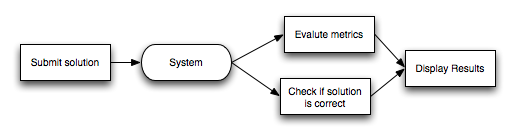
\includegraphics[scale=0.7]{images/arq}
\caption{Simplified System Architecture}
\label{fig:arq}
\end{figure}

As it would be expected, our system allows the creation of new contests, where among other things, we can stipulate the date in which the contest starts and ends, and also it's durations. Several exercises can be added to each contest, either manually, or by submitting one or more xml files. An exercise has a description, a set of languages in which the competitors can solve the exercice, and a set of input's and output's that the program will try to pass.
Having the contest propely created and being available to the competitors, they can register to be a contest participant, and then start submitting their solutions to each of the contest exercises.  





